\documentclass[a4paper,11pt]{article}

\usepackage{graphics}
\usepackage{graphicx}

\begin{document}

\title{Project Proposal}

\author{Fajran Iman Rusadi - 5781574\\
ZhengZhangzheng - 5901995}

\date{}
\maketitle

\section{Background}

Most state of the art sensor networks existing now are designed for a single
application. However, it is expected that many users will need to make
different use of the sensor infrastructure. For instance, a user could be
interested in temperature data on specific intervals, while another user might
want to correlate audio streams coming from microphone arrays. As a
consequence, a sensor network should support multiple applications. An issue
that complicates the matter is, the type of applications that will run on a
sensor network of such scale and time cannot be known beforehand. In our
project, we present our solutions to run different applications on the same
sensor network without one application interfering with other applications, and
the new application can be propagated to all the nodes in the sensor network
easily by means of radio communication.

\section{Implementation Idea}

\subsection{Software Architecture}

\begin{figure}[htbp]
	\centering
	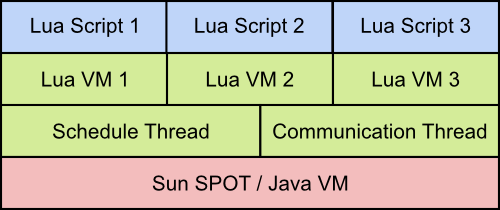
\includegraphics[width=7.5cm]{stack}
	\caption{Component Stack}
	\label{fig:stack}
\end{figure}


The Figure~\ref{fig:stack} above reflects the software architecture of our
implementation. In our implementation, the sensor network will run a virtual
machine to run applications that contains the detailed application logic to
fulfill a certain task in the sensor network.

We will use Lua virtual machine and therefore the application is written in Lua
scripting language. Every time a new Lua script is run, a new Lua virtual
machine is created and the script will be run on top of it. A scheduler will be
written to schedule execution of applications that are being run to guarantee
the isolation from application to application. This scheduler will be run on
its own thread, "Schedule Thread".

To make the applications, that are run on the virtual machine, can access
libraries on the sensor network, some functions in the libraries will be
exported to the virtual machine. In this way, the applications can make
functionalities that are offered by the sensor network.

To ensure the applications can be scheduled and run as expected, a kind of
application framework (or "how the application should be written") will be used
by the applications. All applications that want to be run in this sensor
network have to follow the rules.

Beside scheduling the Lua applications, the main program in the sensor network
will also acts as an application manager and communication handler. It receives
new applications from the network, runs them in the virtual machine, stops the
execution, and also deletes the application. It will also handle the
communication with other sensor networks including the routing function. This
part of the program will be run on a different thread, "Communication Thread".

\subsection{Data Propagation}

We assume there is a base station in the collection of sensor networks that
will acts as the main node. This is the node that will initially send new
applications to the network to be installed and run on every nodes of sensor
networks. This is also the node that will be the final destination of all
result data sent by the other sensor networks.

To propagate a data to all sensor network, each node will have a forwarding and
routing function. These functions are implemented to make sure a data packet
that is sent from the base station can reach all other nodes and all packets
that contain data result from all nodes can be sent back to the base station.

\end{document}

